\documentclass[conference]{IEEEtran}
\renewcommand\IEEEkeywordsname{Palabras clave:}
\IEEEoverridecommandlockouts
\usepackage[utf8]{inputenc}                   % Para escribir tildes y eñes
\usepackage[spanish]{babel}                   % Para que los títulos de figuras, tablas y otros estén en español


%cargar plantilla

% The preceding line is only needed to identify funding in the first footnote. If that is unneeded, please comment it out.
%cargar paquetes(usepackage)
\usepackage{cite}
\usepackage{amsmath,amssymb,amsfonts}
\usepackage{algorithmic}
\usepackage{graphicx}
\usepackage{textcomp}
\usepackage{xcolor}
\usepackage{listings}

%sangria y margenes de la hoja
\def\BibTeX{{\rm B\kern-.05em{\sc i\kern-.025em b}\kern-.08em
    T\kern-.1667em\lower.7ex\hbox{E}\kern-.125emX}}
   


\addto\captionsspanish{\renewcommand{\tablename}{Tabla}}					% Cambiar nombre a tablas
\addto\captionsspanish{\renewcommand{\listtablename}{Índice de tablas}}		% Cambiar nombre a lista de tablas
\usepackage{geometry}                         
\geometry{left=18mm,right=18mm,top=21mm,bottom=21mm} % Tamaño del área de escritura de la página
\usepackage{ucs}
\usepackage{amsmath}      % Los paquetes ams son desarrollados por la American Mathematical Society
\usepackage{amsfonts}     % y mejoran la escritura de fórmulas y símbolos matemáticos.
\usepackage{amssymb}
\usepackage{graphicx}     % Para insertar gráficas
\usepackage[lofdepth,lotdepth]{subfig}	% Para colocar varias figuras
\usepackage{unitsdef}	  % Para la presentación correcta de unidades
\usepackage{pdfpages}   %incluir paginas de pdf externo, para los anexos
\usepackage{appendix}   %para los anexos
\renewcommand{\unitvaluesep}{\hspace*{4pt}}	% Redimensionamiento del espacio entre magnitud y unidad
\usepackage[colorlinks=true,urlcolor=blue,linkcolor=black,citecolor=black]{hyperref}     % Para insertar hipervínculos y marcadores
\usepackage{float}		% Para ubicar las tablas y figuras justo después del texto
\usepackage{booktabs}	% Para hacer tablas más estilizadas
\batchmode
\bibliographystyle{plain} 
\pagestyle{plain} 
\pagenumbering{arabic}
\usepackage{lastpage}
\usepackage{fancyhdr}	% Para manejar los encabezados y pies de página
\pagestyle{fancy}		% Contenido de los encabezados y pies de pagina
\usepackage{multicol}   % Para varias columnas

\lhead{Ing. Tecnologías de la Información y Comunicaciones}
\rhead{Proyecto Integrador} 
\lfoot{ITICS}
\cfoot{\thepage\ de \pageref{LastPage}}
\rfoot{ITSOEH}

%sangria y margenes de la hoja
\def\BibTeX{{\rm B\kern-.05em{\sc i\kern-.025em b}\kern-.08em
    T\kern-.1667em\lower.7ex\hbox{E}\kern-.125emX}}
    
\begin{document}%inicio del documento

%plantilla imprimir codigo Java
\lstnewenvironment{javaCode}[1][]
{\lstset{
    language=Java,
    basicstyle=\footnotesize\ttfamily,
    numbers=left,
    numberstyle=\tiny,
    stepnumber=1,
    numbersep=5pt,
    keywordstyle=\color{blue},
    commentstyle=\color{gray},
    stringstyle=\color{purple},
    breaklines=true,
    breakatwhitespace=true,
    tabsize=4,
    showspaces=false,
    showstringspaces=false,
    frame=single,
    captionpos=b,
    #1
}}
{}

% --- Datos de la práctica y de los alumnos  ------

\title{

\includegraphics[width=6cm]{imagen/LOGO-SEP.png}
\includegraphics[width=5cm]{imagen/TECNM.png}
\includegraphics[width=4.5cm]{imagen/ITSOEH logo.png}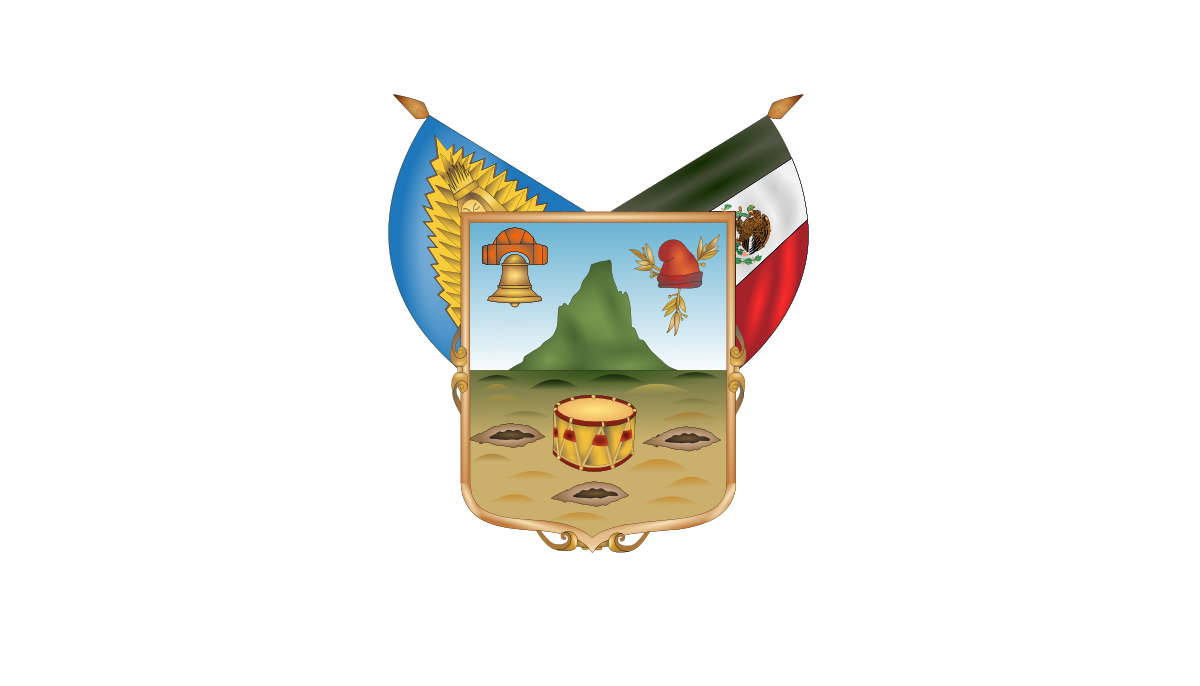
\includegraphics[width=5cm]{imagen/Flag_of_Hidalgo.svg.png}
\\ \vspace*{0.6cm} {\Large Instituto Tecnológico Superior del Occidente del Estado de Hidalgo} \\
  \vspace*{0.2cm}
  \Large Ingeniería en Tecnologías de la Información y Comunicaciones  \\  
  \vspace*{0.5cm}  
  {\it \huge Proyecto Integrador} \\
  {\normalsize Software de resolución de problemas de ingeniería}\\
  {\vspace{1cm} \large \textbf{Coordinador del proyecto:}\\ Dr. Francisco Javier Cuadros Romero}\\
  \vspace{1cm}
  {\large \textbf{Integrantes del equipo:}}
  \vspace{0.5cm}
  }
%titulo del docuemento

\author
{\IEEEauthorblockN{1\textsuperscript{er} Cedillo Ramírez Jesús Emmanuel}
\IEEEauthorblockA{\textit{Estudiante de ITIC´s} \\
\textit{ITSOEH}\\
Progreso de Obregón, HGO. \\
230110478@itsoeh.edu.mx}
\and

\IEEEauthorblockN{2\textsuperscript{do} Gómez Ángeles Evelin}
\IEEEauthorblockA{\textit{Estudiante de ITIC´s} \\
\textit{ITSOEH}\\
Tezontepec de Aldama, HGO. \\
230110617@itsoeh.edu.mx}
\and

\IEEEauthorblockN{3\textsuperscript{er} Gonzaga López Luis Fernando}
\IEEEauthorblockA{\textit{Estudiante de ITIC´s} \\
\textit{ITSOEH}\\
Tlahuelilpan, HGO. \\
230110528@itsoeh.edu.mx}
\and

\IEEEauthorblockN{4\textsuperscript{to} González Calva Yael}
\IEEEauthorblockA{\textit{Estudiante de ITIC´s} \\
\textit{ITSOEH}\\
Progreso de Obregón, HGO. \\
230110582@itsoeh.edu.mx}
\and

\IEEEauthorblockN{5\textsuperscript{to} Jarquín Contreras Kevin Ichiro}
\IEEEauthorblockA{\textit{Estudiante de ITIC´s} \\
\textit{ITSOEH}\\
Mixquiahuala, HGO. \\
230110949@itsoeh.edu.mx}
\and

\IEEEauthorblockN{6\textsuperscript{to} López Paz Gustavo}
\IEEEauthorblockA{\textit{Estudiante de ITIC´s} \\
\textit{ITSOEH}\\
Progreso de Obregón, HGO. \\
230110531@itsoeh.edu.mx}

}
\vspace{2cm}
\maketitle%termina el titulo
\clearpage
\onecolumn
\tableofcontents

\clearpage
\twocolumn
\begin{abstract}
    Pasado el tiempo desde inicio de semestre Agosto-Diciembre 2023, se han abarcado diferentes temas aprendidos con diferentes metodologías correspondientes a cada uno de los docentes de las siete materias que contiene el primer semestre de ingeniería en Tecnologías de la Información y Comunicaciones, dentro de estos temas se escogieron tres problemas de Cálculo Diferencial y tres problemas de Matemáticas Discretas, desarrollándolos con conocimientos adquiridos en Fundamentos de Programación, y subiendo la solución de estos mismos en un repositorio de GitHub, y haciendo el siguiente informe con el proceso de solución de cada uno de los ejercicios, resueltos con uso de la metodología de las 6D's.
\end{abstract}

\begin{IEEEkeywords}
    Matemáticas, conocimientos, problemas, solución, metodología.
\end{IEEEkeywords}

\section{Introducción}
En el siguiente documento se presentan seis problemas de primer semestre de ingeniería: el primero de ellos es encontrar la ecuación de la recta dados dos puntos en el plano cartesiano $(x_1, y_1)$ y $(x_2, y_2)$, obteniendo la pendiente m que se define como $ m = (y_2 - y_1)/(x_2 - x_1) $ para arrojar el resultado de la ecuación de la recta de la forma $ y= m x + b $ donde b es el punto de intersección con el eje y; el segundo problema es encontrar el valor de las raíces de una ecuación cuadrática o ecuación de segundo grado de la forma $ ax^2 +bx + c = 0 $, por medio de la fórmula general que se define como $ x = (-b\pm \sqrt{b^2-4ac})/(2a) $ donde $a, b y c$ son los coeficientes que acompañan a la ecuación cuadrática; el tercer problema es arrojar si un punto dado del plano cartesiano está dentro o fuera de una circunferencia con centro fuera del origen comparando el valor del radio de la circunferencia y la distancia que hay entre el punto dado con el punto que marca el centro de la circunferencia, esta distancia la encontraremos con la fórmula de distancia entre dos puntos en el plano cartesiano que se define como $d=\sqrt{(x_2-x_1)^2+(y_2-y_1)^2}$, y así de esta manera resolver este problema; el cuarto problema es encontrar el número binario correspondiente a un número decimal dado por el usuario el cual tiene un método de división sucesiva para encontrar el binario del decimal; el quinto problema es inverso al problema anterior el cual consiste en encontrar el valor en numeración decimal de un número binario dado por el usuario, usando un método de potenciación de base dos y exponente con valor de posición del dígito del número binario comenzando de derecha a izquierda, por muy similar que se noten estos dos últimos problemas tienen una metodología diferente para su solución; el sexto y último problema consiste en encontrar una expresión booleana que genere las salidas en una tabla de $n$ bits, donde $n$ será el valor dado por el usuario.\\

Estos seis problemas mencionados brevemente fueron analizados y resueltos con una metodología en común que es la metodología de las 6D's: Definición del problema, donde mencionamos información acerca del tema que contiene el problema; Descripción del problema, donde solo hacemos mención del problema a resolver; Diseño de solución, donde se hace un análisis de como resolver el problema y dar la matemática que contiene cada uno de estos; Desarrollo de solución, donde se da a detalle y por paso la solución de estos agregando el código hecho en lenguaje de programación JAVA; Depuración y pruebas, donde se agregan tablas de corrida del código con datos dados por el usuario y el dato arrojado por el programa; y Documentación, la cual consiste en el siguiente informe.


\section{Objetivos}
\subsection{Objetivo General}
\begin{itemize}
    \item Desarrollar un software en lenguaje JAVA para la solución útil y precisa de problemas matemáticos y de ingeniería, que permita a los usuarios realizar cálculos y análisis numéricos de manera efectiva.
\end{itemize}

\subsection{Objetivos específicos}
\begin{enumerate}
    \item Comprender la ecuación de la recta, la fórmula general y la distancia entre dos puntos, para resolver problemas matemáticos relacionados con el álgebra y geometría, y aplicados a la ingeniería.
    \item Comprender y aplicar los métodos de conversión de numeración binaria a numeración decimal, y viceversa.
    \item Aplicar los conceptos de tablas de verdad para analizar expresiones lógicas.
\end{enumerate}

\section{Problemas}
\subsection{Ecuación de la recta}
\subsubsection{Definición del problema}
Se trata de una noción de la geometría que refiere a la línea unidimensional que, formada por una cantidad infinita de puntos, se prolonga en una misma dirección.
\begin{enumerate}
    \item Una línea recta es el lugar geométrico en un plano formado por una sucesión de puntos que tienen la misma dirección. Dados dos puntos diferentes, sólo una recta pasa por esos dos puntos.
    \item Es el lugar geométrico de los puntos de un plano, de los cuales al tomar dos cualesquiera, el valor de la pendiente m, es siempre constante.
    \item Es el lugar geométrico formado por un polinomio de primer grado de la forma $y= mx + b$.
    \item Es el lugar geométrico obtenido al unir dos puntos, tal que la distancia recorrida, es la más corta posible.
    \end{enumerate}
\subsubsection{Descripción del problema}
Dados 2 puntos A y B con coordenadas $(x_1, y_1)$ y $(x_2,y_2)$ respectivamente. Regresar la ecuación de la recta y el ángulo interno a que se forma entre el eje horizontal y la recta.
\subsubsection{Diseño de solución}
En la ecuación de la recta si dos puntos distintos $P(x_{1},y_{1})$ y $Q(x_{2},y_{2})$ se ubican en la curva $y=f(x)$, la pendiente de la recta secante que une los dos puntos es: 
\begin{equation}
    m_{secc} = \frac{y_{1}-y_{2}}{x_{1}-x_{2}} = \frac{f(x_{1})-f(x_{2})}{x_{1}-x_{2}}
\end{equation}
Para identificar la intersección en el eje vertical se utiliza cualquiera de los dos puntos para este caso se utilizó $P(x_{1},y_{1})$ de la siguiente forma:
\begin{equation}
    y = mx + b
\end{equation}

\begin{figure}[h!]
    \centerline{\includegraphics[width=6cm]{imagen/GráficaEcuacionRecta.png}}
    \caption{Gráfica de la ecuación de la recta}
    \label{fig}
\end{figure}
Utilizando este método, puedes encontrar la ecuación de la recta a partir de dos puntos dados. Recordando que si dos puntos son idénticos, la recta será una línea vertical \cite{articuloRecta}.
Y para calcular el ángulo de dicha pendiente se usa: 

\begin{equation}
    \sphericalangle=\arctan(m)
\end{equation}


\subsubsection{Desarrollo de solución}
\begin{enumerate}
    \item El algoritmo de solución implementado en el lenguaje JAVA empieza por la entrada de los valores $P(x_{1},y_{1})$ y $Q(x_{2},y_{2})$ solicitando que sean separados por una coma.
    \begin{javaCode}
    Scanner punto = new Scanner(System.in);
            
    //solicitar puntos
    System.out.println(
    """
    Ingrese las coordenadas (x,y) separadas 
    por una coma(,) del punto 1:
    """);
    String [] puntoUno = punto.nextLine().split(",");
            
    System.out.println(
    """
    Ingrese las coordenadas (x,y) separadas 
    por una coma(,) del punto 2: """);
    String [] puntoDos = punto.nextLine().split(",");
            
    punto.close();
    \end{javaCode}

    \item Después de ingresar los valores, se obtienen los valores ingresados para después convertirlos de valores de cadena a valores enteros, para esto se aplicó el siguiente método de conversión.

    \begin{javaCode}
    String[] coordenadasArrayPunto1 = coordenadasPunto1.split(",");
    String[] coordenadasArrayPunto2 = coordenadasPunto2.split( ",");
            
    //obtener coordenadas X y Y
    int coordenadaX1 = Integer.parseInt(coordenadasArrayPunto1[0].
    trim());
    int coordenadaY1 = Integer.parseInt(coordenadasArrayPunto1[1].
    trim());
            
    int coordenadaX2 = Integer.parseInt(coordenadasArrayPunto2[0].
    trim());
    int coordenadaY2 = Integer.parseInt(coordenadasArrayPunto2[1].
    trim());
            
    System.out.println("Coordenada X1: " + coordenadaX1);
    System.out.println("Coordenada Y1: " + coordenadaY1);
            
    System.out.println("Coordenada X2: " + coordenadaX2);
    System.out.println("Coordenada Y2: " + coordenadaY2);
    \end{javaCode}

    \item Luego se calcula la pendiente m utilizando la fórmula de la pendiente\cite{articuloRecta}.

    \begin{javaCode}
        double m = (coordenadaY2 - coordenadaY1)/(coordenadaX2 - coordenadaX1);
    \end{javaCode}

    \item A continuación se calcula el término b de la fórmula de intersección.

    \begin{javaCode}
        double b = coordenadaY1 - m * coordenadaX1;
    \end{javaCode}

    \item Por último calculamos el ángulo interno que se forma entre el eje horizontal y la recta pendiente.
    
    \begin{javaCode}
        double anguloRadianes = Math.atan(m);
        double anguloGrados = anguloRadianes * (180/Math.PI);
    \end{javaCode}

    \item Obteniendo finalmente el resultado de la intersección de la recta y su ángulo interno que se formó.
\end{enumerate}
\subsubsection{Depuración y pruebas}
En la tabla 1 se muestran los resultados obtenidos al compilar el código.\\
\begin{table}[!ht]
\label{T:equipos}
\begin{center}
\begin{tabular}{| c | c | c | c | c | c | c |}
\hline
\textbf{$x_1$} & \textbf{$x_2$} & \textbf{$y_1$} & \textbf{$y_2$} & \textbf{Pendiente} & \textbf{Inclinación} & \textbf{Intersección} \\
\hline
2 & 4 & 4 & 6 & 1 & 45$^o$ & -2 \\
3 & 2 & 4 & 1 & 3 & 71.57$^o$ & -5 \\
2 & 2 & 2 & 2 & 0 & 0$^o$ & 0 \\
1 & 3 & 2 & 4 & 1 & 45$^o$ & 1 \\
\hline
\end{tabular}
\caption{Tabla de corridas.}
\end{center}
\end{table}\\

\subsection{Raíces de una ecuación cuadrática}

\subsubsection{Definición del problema}
La ecuación cuadrática o fórmula cuadrática es utilizada para encontrar las raíces de una ecuación cuadrática de la forma $ax^{2}+bx+c = 0$, la fórmula se compone por 3 parámetros:
\begin{enumerate}
    \item Parámetro ${a}$: Representa la posición del vértice de la parábola en el eje ${Y}$.
    \item Parámetro ${b}$: Representa la posición del vértice en la parábola del eje ${X}$.
    \item Parámetro ${c}$: Representa el punto de intersección de la parábola con el eje ${Y}$.
\end{enumerate}
El uso de esta fórmula es útil cuando se requiere resolver alguna ecuación cuadrática que ya se intentó resolver por distintos métodos o por medio de la factorización, por ello la formula cuadrática es la siguiente:
\begin{equation}
    x = \frac{-b\pm\sqrt{b^2-4ac}}{2a}
\end{equation}
En esta fórmula se toma en cuenta el discriminante que es representado en la fórmula por $b^2-4ac$, el cual determina la naturaleza y el número de soluciones de la ecuación, analizando las propiedades de una ecuación cuadrática y determinar su comportamiento de soluciones reales.\cite{FormulaCuadratica}\\

\begin{figure}[H]
    \centerline{\includegraphics[width= 6cm]{imagen/GráficaFormulaCuadrática.png}}
    \caption{Gráfica de la fórmula cuadrática}
    \label{fig}
\end{figure}

\subsubsection{Descripción del Problema}
Se solicita al usuario que ingrese los tres parámetros $a$, $b$, y $c$, donde estos se evaluarán en un discriminante el cual es $b^2-4ac$, y que al final dependiendo de este se resuelva el resto de la operación de esta fórmula.

\subsubsection{Definición de la solución}
Para tener solución a este problema se consideran 3 posibles respuestas que dependen del discriminante, las cuales son:
\begin{enumerate}
    \item La ecuación tiene dos soluciones sobre el conjunto de los números reales, $x_1$ y $x_2$.
    \item La ecuación solo tiene una solución en el conjunto de los números reales, $x$.
    \item La ecuación no tiene una solución en el conjunto de los números reales, esta se encuentra en el conjunto de los números complejos.
\end{enumerate}

\subsubsection{Diseño de la solución}
Para resolver este problema se requiere que el programa reciba 3 coeficientes de tres parámetros que vendrán de la ecuación cuadrática que se tenga, donde primero se establece el desarrollo del discriminante y por consiguiente la evaluación del discriminante donde determinará si existen dos soluciones, una solución o solución en el conjunto de los complejos.

\subsubsection{Desarrollo de la solución}

\begin{enumerate}
    \item La solución a este problema se diseño un programa el cual se tendrá que ingresar los 3 coeficientes de los parámetros denominados de $a$, $b$, y $c$ para resolver la fórmula cuadrática.
    
    
    \begin{javaCode}
    
        System.out.println("Ingrese el parámetro de a de la ecuación cuadrática");
            double a = in.nextDouble();
            System.out.println("Ingrese el parámetro de b de la ecuación cuadrática");
            double b = in.nextDouble();
            System.out.println("Ingrese el parámetro de c de la ecuación cuadrática");
            double c = in.nextDouble();
            
    \end{javaCode}
    
    \item Por consiguiente primero se resolverá el discriminante, donde el resto de las operaciones de la fámula cuadrática dependerá de este resultado.
    
    \begin{javaCode}
        double discriminante = (Math.pow(b, 2)) - (4*a*c);3
    \end{javaCode}
    
    \item Por último, si el discriminante pasa por la primer condición, se obtendrán 2 soluciones, la segunda condición solo tiene una solución, en caso contrario de todo, no hay una solución posible.
    
    \begin{javaCode}
        if (discriminante > 0) {
                double x1 = (-b + Math.sqrt(discriminante)) / (2 * a);
                double x2 = (-b - Math.sqrt(discriminante)) / (2 * a);
                
                System.out.println("La ecuacion tiene dos soluciones sobre el conjunto de los números reales: \nx1 = "+x1+"\nx2 = "+x2);
            } else {
                if (discriminante==0) {
                    double x = -b/(2*a);
                    System.out.println("La ecuación solo tiene una solución sobre el conjunto de los números reales: \nx = "+x);
                } else {
                    System.out.println("La ecuación no tiene una solución en el conjunto de los números reales,esta se encuentra en los números complejos");
                }
            }
    \end{javaCode}
\end{enumerate}
\subsubsection{Depuración y pruebas}
En la tabla II se muestran los resultados obtenidos al compilar el código.
\vspace{0.8cm}
\begin{table}[!ht]
\label{T:equipos}
\begin{center}
\begin{tabular}{| c | c | c | c | c | c |}
\hline
\textbf{$a$} & \textbf{$b$} & \textbf{$c$} & \textbf{$x_1,x_2$ o $x$}\\
\hline
2 & 10 & 2 & -0.20, -4.79 \\
3 & 4 & 6 & "solución en los números complejos" \\
-5 & 6 & -1 & 0.2,  1.0 \\
7 & 4 & 10 & "solución en los números complejos" \\
1 & -4 & 4 & 2 \\
\hline
\end{tabular}
\caption{Tabla de corridas.}
\end{center}
\end{table}\\

\subsection{Punto dada una circunferencia}

\subsubsection{Definición del problema}
La circunferencia es el lugar geométrico de los puntos del plano que equidistan de un punto fijo llamado centro (C) con coordenadas:
$$C:(x,y)$$
Esta contiene un elemento llamado radio (r) el cual se define como la línea que une el centro con cualquier punto de la circunferencia. La magnitud del radio determinará que tanto se abrirá la circunferencia.\cite{Circunferencia}\\

\subsubsection{Descripción del problema}
Dada una circunferencia con centro en el punto $C$ con coordenadas $(x_1, y_1)$ y radio $r$, evaluar si un punto $T$ con coordenadas $(x_2, y_2)$ está dentro de la circunferencia.\\

\subsubsection{Diseño de solución}
Para darle solución a este problema se analizaron los casos que pueden ocurrir dentro de este, encontrando tres casos diferentes:
\begin{enumerate}
    \item El punto T se encuentra dentro de la circunferencia.
    \item El punto T se encuentra fuera de la circunferencia.
    \item El punto T se encuentra sobre la circunferencia.
\end{enumerate}
Para determinar cual de los tres casos se cumplen se tiene que encontrar primero la distancia que hay entre el centro de la circunferencia y el punto T.\\
Usando la fórmula para la distancia $d$ entre dos puntos en el plano cartesiano que se define como:
\begin{equation}
    d = \sqrt{(x_2-x_1)^2+(y_2-y_1)^2}
\end{equation}
Con la ecuación 5 encontramos la magnitud entre el punto T y el centro de la circunferencia.\\
Se hace la comparación entre la distancia $d$ que hay entre ambos puntos, con el valor del radio de la circunferencia:
\begin{enumerate}
    \item Si d > r entonces el punto T se encuentra fuera de la circunferencia.
    \item Si d < r entonces el punto T se encuentra dentro de la circunferencia.
    \item Si d = r entonces el punto T se encuentra sobre la misma circunferencia.
\end{enumerate}
Con esto entendido se procede a desarrollar la solución en lenguaje de programación Java.\\

\subsubsection{Desarrollo de la solución}
\begin{enumerate}
    \item Se le solicita al usuario las coordenadas en x y en y del centro de la circunferencia.
    \begin{javaCode}
        System.out.println("Ingrese el valor de la coordenada en x del centro de la circunferencia: ");
        double Cx = entrada.nextDouble();
        System.out.println("Ingrese el valor de la coordenada en y del centro de la circunferencia: ");
        double Cy = entrada.nextDouble();
    \end{javaCode}
    \item Se le solicita al usuario los valores de las coordenadas en x y en y del punto T a evaluar.
    \begin{javaCode}
        System.out.println("Ingrese el valor de la coordenada en x del punto T: ");
        double Tx = entrada.nextDouble();
        System.out.println("Ingrese el valor de la coordenada en y del punto T: ");
        double Ty = entrada.nextDouble();
    \end{javaCode}
    \item Se le solicita al usuario el valor del radio de la circunferencia.
    \begin{javaCode}
        System.out.println("Ingrese el valor del radio de la circunferencia");
        double r = entrada.nextDouble();
    \end{javaCode}
    \item Se procesa la información ingresada por el usuario para obtener la distancia entre el centro de la circunferencia y el punto T.
    \begin{javaCode}
        double v1 = Math.pow((Tx-Cx), 2);
        double v2 = Math.pow((Ty-Cy), 2);
        double v3 = v1+v2;
        double d = Math.sqrt(v3);
    \end{javaCode}
    \item Se compara la distancia obtenida con el radio, haciendo uso del if, else if y else para saber que caso ocurre e imprimirlo al usuario.
    \begin{javaCode}
        if (d>r){
            System.out.println("El punto T con coordenadas ("+Tx+", "+Ty+") se encuentra fuera de la circunferencia con centro en ("+Cx+", "+Cy+") y radio "+r);
        }else if (d<r){
            System.out.println("El punto T con coordenadas ("+Tx+", "+Ty+") se encuentra dentro de la circunferencia con centro en ("+Cx+", "+Cy+") y radio "+r);
        }else if (d==r){
            System.out.println("El punto T con coordenadas ("+Tx+", "+Ty+") se encuentra sobre la circunferencia con centro en ("+Cx+", "+Cy+") y radio "+r);
        }
    \end{javaCode}
\end{enumerate}

\subsubsection{Depuración y pruebas}
A continuación, en la tabla II se muestran los resultados de prueba al compilar el código.\\

\begin{table}[!ht]
\label{T:equipos}
\begin{center}
\begin{tabular}{| c | c | c | c | c | c |}
\hline
\textbf{$C_x$} & \textbf{$C_y$} & \textbf{$T_x$} & \textbf{$T_y$} & \textbf{$r$} & \textbf{Fuera/Dentro/Sobre}\\
\hline
4 & 4 & 5 & 5 & 1 & Fuera \\
3 & 4 & 6 & 8 & 5 & Sobre \\
-5 & 6 & -1 & 2 & 15 & Dentro \\
0 & 0 & 0 & 5 & 5 & Sobre\\
3 & 7 & 9 & 2 & 6 & Dentro\\
\hline
\end{tabular}
\caption{Tabla de corridas.}
\end{center}
\end{table}

\subsection{Conversión decimal a binario}

\subsubsection{Definición del problema}
El sistema decimal, es un sistema de numeración posicional en el que las cantidades se representan utilizando como base el número diez, por lo que se compone de diez dígitos diferentes: 0, 1, 2, 3, 4, 5, 6, 7, 8, 9.
El valor de cada dígito está asociado a la posición que ocupa: unidades, decenas, centenas, millares, etc. 
Un sistema binario utiliza sólo dos dígitos: 0 y 1. El valor de cada posición se obtiene de una potencia de base dos, elevada a un exponente igual a la posición del dígito menos uno.\cite{SistemaDecimal}\\
\subsubsection{Descripción del Problema}
Dado un número decimal entero positivo o negativo regresar su equivalente en binario.
\subsubsection{Diseño de solución}
Para darle solución a este problema de un número entero decimal a binario, se debe utilizar el método de división sucesiva. Este método consiste en dividir el número decimal entre 2 y anotar el residuo. Luego, se divide el cociente obtenido entre 2 y se anota el nuevo residuo. Este proceso se repite hasta obtener un cociente igual a 0. Los residuos obtenidos, leídos de abajo hacia arriba, forman la representación binaria del número decimal. Desarrollando un código en Java, en donde el usuario ingrese un número entero decimal y obtenga como resultado su número binario.
\subsubsection{Desarrollo de la solución}
\begin{enumerate}
    \item En el programa que se desarrolló en Java, el usuario tiene que ingresar un número entero decimal positivo siendo este el valor primordial para que se lleve a cabo la conversión a binario.
    \begin{javaCode}
        System.out.println("Ingrese un número entero decimal positivo");
        int númeroDecimal=entrada.nextInt();
    \end{javaCode}
    \item Se utiliza la estructura en cascada, en dónde se verifica si el número no es negativo e inicializa una cadena para almacenar el número binario y si el número decimal es igual a 0, se asigna "0" a la variable número binario.
    En caso de que el número no sea negativo, se utiliza un bucle while para convertir el número decimal a su representación binaria. Se calcula el residuo de la división del número decimal entre 2 y se guarda en la variable residuo. Se concatena el residuo al inicio de la cadena número binario y después se divide el número decimal entre 2 y se actualiza el valor de número decimal. Finalmente se imprime el número binario resultante.\\
    \begin{javaCode}
       if (númeroDecimal<0) {
       System.out.println("El número debe ser entero no negativo");
       return;
       }
       String númeroBinario="";
       if (númeroDecimal==0) {
           númeroBinario="0";
        } else {
        while (númeroDecimal>0) {
        int residuo=númeroDecimal%2;
        númeroBinario=residuo+númeroBinario;
        númeroDecimal=númeroDecimal/2; 
        }
        }
        System.out.println("El número binario equivalente es:" + númeroBinario);
        
    \end{javaCode}
    \item Por lo tanto, obtenemos el resultado de la conversión de el número entero decimal en binario.
\end{enumerate}
\subsubsection{Depuración y pruebas}
A continuación en la tabla 4 se muestran resultados arrojados por el código.
\begin{table}[!ht]
\label{T:equipos}
\begin{center}
\begin{tabular}{| c | c | c | c | c | c |}
\hline
\textbf{Número} & \textbf{Número decimal} & \textbf{Número binario}\\
\hline
1 & 222 & 11011110 \\
2 & 338 & 101010010 \\
3 & 110 & 1101110 \\
\hline
\end{tabular}
\caption{Tabla de corridas.}
\end{center}
\end{table}\\

\subsection{Conversión binario a decimal}


\subsubsection{Definición del problema}

El código binario se basa en un sistema de dos elementos constituido por el cero y uno,el código binario es una secuencia de dígitos que representa el lenguaje que utilizan los equipos con circuitos digitales para procesar información y comandos.  
\\
El sistema binario es la base de la tecnología digital, cualquier dispositivo que tenga circuitos integrados (chips) es posible gracias a este sistema numérico.
\\
El sistema binario se emplea por los ordenadores generalmente, tanto por los componentes hardware como por el software.\cite{SistemaBinario}\\

\begin{figure}[H]
    \centerline{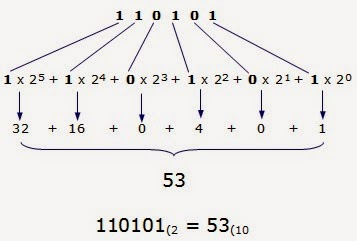
\includegraphics[width= 6cm]{imagen/binario-a-decimal-java.jpg}}
    \caption{Ejemplo Binario-Decimal}
    \label{fig}
\end{figure}

\subsubsection{Descripción del problema}

Dado un número binario de $n$ bits regresar su equivalente en decimal.\\

\subsubsection{Diseño de solución}

El proceso para convertir un número binario a decimal es un método diferente.

Consta de numerar los dígitos de derecha a izquierda comenzando desde cero, a cada número se le asigna la correspondiente potencia base 2 y al final se suman las potencias.\\

Lo primero que se debe realizar es ubicar una serie de potencias de dos que es la base del sistema binario, cuyo exponente va aumentando a medida que cambiamos la posición de derecha a izquierda, después se multiplica cada dígito del número binario por el resultado de la potencia, después se deben sumar los resultados para poder encontrar el número decimal.\\

\subsubsection{Desarrollo de la solución del problema}

\begin{enumerate}
    \item Se diseño un diagrama de flujo para poder realizar un programa en JAVA en el cual pide ingresar un número binario.
    \begin{javaCode}
     //ENTRADA
     System.out.println("Ingresa un numero binario");
            String numeroBin = in.nextLine();
            int longitud = numeroBin.length();
            int numeroDecimal = 0;
    \end{javaCode}
    \item A base de una codificación te mostrará como resultado el número decimal correspondiente al número binario ingresado.
     \begin{javaCode}
     //PROCESO
     for (int i = 0; i < longitud; i++) {
                
                char digito = numeroBin.charAt(i);
                
                //verificacion si es 0 o 1
                if (digito == '0') {
                    numeroDecimal *= 2;
                } else if(digito == '1') {
                    numeroDecimal = (numeroDecimal * 2) + 1;
                } else {
                    System.out.println("El numero binario ingresado no es valido");
                    return;
                }
            }
            
     \end{javaCode}
    \item Y al final se mirará reflejado el número decimal correspondiente al número binario solicitado.
    \begin{javaCode}
    //SALIDA
        System.out.println("El numero decimal equivalente es " + numeroDecimal);
    \end{javaCode}
 \end{enumerate}
\subsubsection{Depuración y pruebas}
A continuación en la siguiente tabla 5 se presentan los resultados de la prueba de compilación del código.

\begin{table}[!ht]
\label{T:equipos}
\begin{center}
\begin{tabular}{| c | c | c | c | c | c |}
\hline
\textbf{Número de corrida} & \textbf{Número binario} & \textbf{Número decimal}\\
\hline
1 & 10101 & 21 \\
2 & 1110001 & 113 \\
3 & 101010111 & 343 \\
\hline
\end{tabular}
\caption{Tabla de corridas.}
\end{center}
\end{table}\\




\subsection{Tabla de verdad usando el teorema booleano}

\subsubsection{Definición del problema}
Las tablas de verdad son instrumentos de la lógica que permiten conocer los valores de verdad de proposiciones compuestas teniendo en cuenta las posibles interpretaciones de las proposiciones simples que la conforman.
Algo que tener en cuenta es que el número de filas de la tabla de verdad será igual a $2^n$ más la cabecera, donde n es el número de proposiciones simples (que podemos llamar variables). Los pasos para crear la tabla podemos resumirlos así:
\begin{enumerate}
    \item Calcular el número de filas que tendrá la tabla de verdad. Este es igual a $2^n$ más la cabecera, donde n es el número de proposiciones simples.
    \item Calcular el número de columnas que tendrá la tabla. Este es igual a el número de proposiciones simples más la cantidad de conectores lógicos que aparecen en la expresión, contando cada repetición de ellos.
    \item Desglosar la proposición compuesta en la cabecera teniendo en cuenta la jerarquía de los conectores. En las primeras columnas irán las proposiciones simples y en la última irá la proposición original.
    \item Escribir en las filas todas las posibles interpretaciones de las proposiciones simples. Por ejemplo, si se trata de dos proposiciones, existen cuatro interpretaciones posibles, lo veremos más adelante con los ejemplos.
    \item Completar el resto de la tabla teniendo en cuenta las tablas de verdad de los conectores lógicos. La última columna, la de la proposición original que analizamos, nos dirá su valor de verdad de acuerdo a las posibles interpretaciones. \cite{TablasdeVerdad}
\end{enumerate}
\subsubsection{Descripción del problema}
Dada una tabla de verdad de "n" bits generar la expresión booleana que genere de manera fidedigna las salidas de esta tabla.

\subsubsection {Diseño de solución}

Este sistema consolida los valores de verdad de todas las combinaciones de premisas y operadores lógicos en un solo lugar en columna. De esta manera, evita que tengas que “calcular” manualmente la conclusión de premisas falsas y verdaderas, muestran todos los posibles escenarios y condiciones de valores de entrada para una operación lógica y su resultado correspondiente, normalmente se utilizan los valores 1 y 0 donde 1 es verdadero y 0 es falso. 
\\
Su función base es mostrar cómo funcionan un circuito electrónico y los programas de una computadora, siendo también un pilar de la lógica proposicional.\\
También la tabla de verdad tiene sus funciones mas importantes como :
\begin{enumerate}
 \item Representan relaciones lógicas.
 \item Analizan todas las combinaciones posibles de valores.
 \item Ayudan a deducir conclusiones lógicas.
 \item Evalúan comportamiento de sistemas ante diferentes entradas.
 \item Mejoran la eficiencia de algoritmos en programación.
\end{enumerate}
También para la correcta elaboración del programa referente a la tabla de verdad se utiliza lo que es el teorema booleano donde: 
\begin{enumerate}
    \item $x * 0 = 0 $
    \item $x * 1 = x$
    \item $x * x = x $
    \item $x .* x´= 0$
    \item $x + 0 = x$
    \item $x + 1 = 1$
    \item $x + x = x$
    \item $x + x´= 0$
\end{enumerate}

Se hizo un código donde se tiene la opción de ingresar la cantidad de bits que uno quiera para eso debemos tener como ingresar la cantidad de bits que deseas para poder elaborar la tabla de valores.
\subsubsection {Desarrollo de solución}
\begin{enumerate}
    \item Para poder ejecutar el problema el código del programa se realizo en el lenguaje de programación java.
    \begin{javaCode}
     import java.util.Scanner;
    public class tabla_de_verdad {
        public static void main(String[] args) {
            Scanner valor=new Scanner (System.in);
            System.out.println("ingresa el numero de bits");
           int numVariables = valor.nextInt(); 
          if(numVariables < 5 ){
            generateTruthTable(numVariables);
        }else{
                System.out.println("Numero fuera de rango permitido :(");
    }
        }
        public static void generateTruthTable(int numVariables) {
            int numRows = (int) Math.pow(2, numVariables);      
            for (int i = 0; i < numVariables; i++) {
                System.out.print("Var" + (i + 1) + "\t");
            }
            System.out.println("Result");
            for (int i = 0; i < numRows; i++) {
                for (int j = numVariables - 1; j >= 0; j--) {
                    int value = (i / (int) Math.pow(2, j)) % 2;
                    System.out.print(value + "\t");
                }
                boolean result = calculateLogicOperation(i, numVariables);
                System.out.println(result ? "1" : "0");
            }
        }
        public static boolean calculateLogicOperation(int row, int numVariables) {
    
            boolean var1 = ((row >> 2) & 1) == 1;
            boolean var2 = ((row >> 1) & 1) == 1;
            boolean var3 = (row & 1) == 1;
            return var1 && var2 && var3;
        }
    }
    
     \end{javaCode}
\end{enumerate}
Para obtener el resultado en expresión booleana primero se debé de modificar una fila como ejemplo en la columna a se modifican alas filas que serían del 1 al 8, porque ocho buenos porque  es la cantidad de filas que la columna la tiene.
 Quiero modificar la fila solo pones el número que corresponda, vas a quieres modificar la fila 2 donde la primera es 0 se cambia a 1 eso varía donde puedes iniciar con 1 y cambia a 0 o viceversa, después de modificar los números que quieras modificar, ya después te dará la ecuación booleana
 
 Ingrese el número de la fila que desea cambiar el resultado a 1 (1-8) o ingrese 0 para finalizar: 0
Expresiones booleanas al finalizar:
A' + B' + C'
A' + B' + C
A' + B + C
A + B' + C
A + B + C'
A + B + C.

Expresión booleana final: (A' + B' + C') + (A' + B' + C) + (A' + B + C) + (A + B' + C) + (A + B + C') + (A + B + C)
\\

\subsubsection {Depuración y pruebas}
En la tabla 6 se muestra un resultado obtenido por el código.
\begin{table}[!ht]
\label{T:equipos}
\begin{center}
\begin{tabular}{| c | c | c | c | c |}
\hline
 \textbf{A} &  \textbf{B} & \textbf{B} & \textbf{RESULTADO}\\
\hline
 0 & 0 & 0 & 1\\
 0 & 0 & 1 & 1 \\
 0 & 1 & 0 &  0\\
 0 & 1 & 1 & 1 \\
 1 & 0 & 0 & 0 \\
 1 & 0 & 1 & 1 \\
 1 & 1 & 0 & 1  \\
 1 & 1 & 1 & 1 \\
\hline
\end{tabular}
\caption{Tabla de corridas.}
\end{center}
\end{table}\\

 

\clearpage
\section{Conclusión}
Con cada uno de los problemas que se resolvieron, se logró una mejor capacitación en distintas áreas como el uso del cálculo diferencial, las búsquedas con números binarios y encontrar sus expresiones booleanas, así como principalmente se desarrolló una mejor comprensión de como poder trabajar en estas áreas con el uso de la programación y mejorar una mejor lógica de desarrollo, al igual de como poder incluir herramientas para trabajar de una manera remota y muy eficiente para poder trabajar mejor en equipo.

\section{Agradecimientos}
 Como equipo mostramos nuestro agradecimiento a cada uno de nuestros docentes de cada una de las materias que contiene el primer semestre de Ingeniería  en Tecnologías de la Información y Comunicaciones, específicamente al \textbf{Mtro. José Martín Oropeza Méndez} quien con entusiasmo nos impartió la asignatura de Matemáticas Discretas I, al \textbf{Ing. Giovany Humberto Neri Pérez} quien con sus conocimientos en matemáticas nos impartió la asignatura de Calculo Diferencial, a la \textbf{Mtra. Silvia Sánchez Bautista} quien con alegría nos impartió la asignatura de Ética, a la \textbf{Lic. Irais López Rojo} quien con su aprendizaje en enseñanza de la segunda lengua nos impartió la asignatura de Inglés I, al \textbf{LSC. Agustín Soto Arista} quien nos ayudó a tener un mejor lenguaje y nos impartió la asignatura de Fundamentos de Investigación, al \textbf{Dr. Francisco Javier Cuadros Romero} quien con mucho conocimiento y clases divertidas nos impartió la asignatura de Introducción a las TIC's, y especialmente agradecidos con la \textbf{MGTI. Citlali Azucena Martínez Calva} quien es tutora de nuestro primer semestre en la carrera y, con sus conocimientos y apoyo extra-clase nos impartió la asignatura de Fundamentos de Programación.\\
 Agradecidos con nuestros padres y amigos que nos apoyaron durante la realización de este proyecto.\\
 Gracias a todos.

\begin{thebibliography}{00}
    \bibitem{articuloRecta} 
    Khan Academy, October 20, 2023, Tangent lines and rates of change, https://www.khanacademy.org/math/calculus-all-old/taking-derivatives-calc/using-the-formal-definition-of-derivative-calc/a/tangent-lines-and-rates-of-change.\\
    
    \bibitem{FormulaCuadratica}
    Tutorela. (2021, 16 noviembre). La fórmula cuadrática. Tutorela. https://www.tutorela.es/matematicas/la-formula-cuadratica\\
    
    \bibitem{Circunferencia}
    Gómez, I. P. Y. F. (2019, 29 junio). Ecuación de la circunferencia - [Ordinaria y general. ¡Ejercicios resueltos!]. Álgebra y Geometría Analítica. https://aga.frba.utn.edu.ar/circunferencia/\\

    \bibitem{SistemaDecimal}
    Porto, J. P., & Merino, M. (2021, 26 agosto). Sistema decimal - qué es, definición, importancia y clasificación. Definición.de. https://definicion.de/sistema-decimal/\\

    \bibitem{SistemaBinario}
    Equipo editorial, Etecé. (2022, 2 febrero). Sistema binario - qué es, concepto, aplicaciones y ejercicios. Concepto. https://concepto.de/sistema-binario/\\

    \bibitem{TablasdeVerdad}
    Machado, D. (2023, 4 noviembre). Cómo hacer tablas de verdad: ejercicios resueltos. Flamath. https://flamath.com/tablas-de-verdad\\

\end{thebibliography}
\\

\section{Integrantes}
\subsection{\textbf{Cedillo Ramírez Jesús Emmanuel}}
Un estudiante de ingeniería que desconoce muchos temas de programación pero que muestra interés en poder aprender diversos temas sobre la programación. Nacido en el municipio de Ixmiquilpan, Hgo, con gustos musicales muy diversos, desde pequeño demostró un interés en temas relacionados con audio, actualmente se encuentra estudiando la carrera de Tecnologías de la Información y Comunicación en el Instituto Superior del Occidente del Estado de Hidalgo, en la cual le ha surgido el interés por el tema de ciberseguridad.

\href{https://github.com/EmmanuelCR23}{GitHub de Emmanuel}\\

\subsection{\textbf{Gómez Ángeles Evelin}}
Una estudiante de ingeniería emocionada por aprender de tecnología y todo lo relacionado con ella. Sus intereses radican en aprender más sobre las diferentes tecnologías y sus aplicaciones en el mundo actual, además de que aspira a adquirir nuevas habilidades de programación para poder diseñar y desarrollar una aplicación que sea útil y beneficie a las personas.

\href{https://github.com/EvelinAngeles06}{GitHub de Evelin}\\

\subsection{\textbf{Gonzaga López Luis Fernando}}
Un estudiante de ingeniería apasionado por la ciencia, la tecnología y las matemáticas. Abierto a diferentes gustos musicales. Nacido en el municipio de Tlaxcoapan, Hgo. y actualmente viviendo en el municipio de Tlahuelilpan, Hgo. Desde la niñez mostró interés en computadoras y en resolver problemas matemáticos. Es jugador de baloncesto desde los 10 años. Sus principales principios como persona son la lealtad y la perseverancia. El principal objetivo de Fernando actualmente es completar sus estudios de nivel superior que actualmente está haciendo en el Instituto Tecnológico Superior del Occidente del Estado de Hidalgo en el municipio de Mixquiahuala de Juárez, Hgo.

\href{https://github.com/FerGonzaga}{GitHub de Fernando}\\

\subsection{\textbf{González Calva Yael}}
Un estudiante de Ingeniería que recientemente ha empezado con cariño a la tecnología que se esfuerza por aprender y de apoyar a sus compañeros cuando lo requieran. Nacido en Francisco I. Madero, Hgo. Cuando era pequeño siempre tuvo el amor hacia el deporte, practicando fútbol y baloncesto a la edad de 9 años, de pocos amigos pero muy buenas personas. Actualmente esta estudiando en el Instituto Superior del Occidente del Estado de Hidalgo, su plan en mente es terminar la carrera y adquirir buenas habilidades para desenvolverse de gran manera en el ámbito laboral. 

\href{https://github.com/YaelDoncic}{GitHub de Yael}\\

\subsection{\textbf{Jarquín Contreras Kevin Ichiro}}

Un estudiante que creció en Mixquiahuala, Hgo. parte de su vida, que tiene un interés por las nuevas tecnologías y el funcionamiento de ellas, por el momento trato de enterder el funcionamiento de eso por eso estudio esta ingeniería en el Instituto Tecnológico Superior del Occidente del Estado de Hidalgo , por el momento tiene una meta en esta carrera y es crear una inteligencia artificial para después de eso poder trabajar de lo que estudia, para esto falta mucho, por el momento tendrá que enfocarse en el ahora para poder lograr sus objetivos a corto y largo plazo.

\href{https://github.com/ichirocontreras}{Github de Ichiro}\\

\subsection{\textbf{López Paz Gustavo}}
Un estudiante que creció en Progreso de Obregón, Hgo. Desde pequeño paso por varios problemas de salud que enfrentar pero con apoyo de sus padres logro salir de ellos, en ese transcurso empezó a tomar cariño de algunos deportes como fútbol y el culturismo, al igual ser curioso con la tecnología que vivía en su alrededor. Con el transcurso del tiempo empezó a aprender por su cuenta programación básica y otras herramientas para trabajar. Hoy ahora que estudia en el Instituto Superior del Occidente del Estado de Hidalgo, en la ingeniería en Tecnologías de la Información y Comunicación, donde también se ha interesado en conocer Internet de las cosas y el manejo de Redes.

\href{https://github.com/Gustavo1Lopez2Paz}{Github de Gustavo}\\

\end{document}